\chapter{Image Processing}
%TC:ignore

\label{appendix:image_processing}

\section{Pre-blue lined image}
\label{processing:pre-line}
\begin{figure}[H]
  \centering
  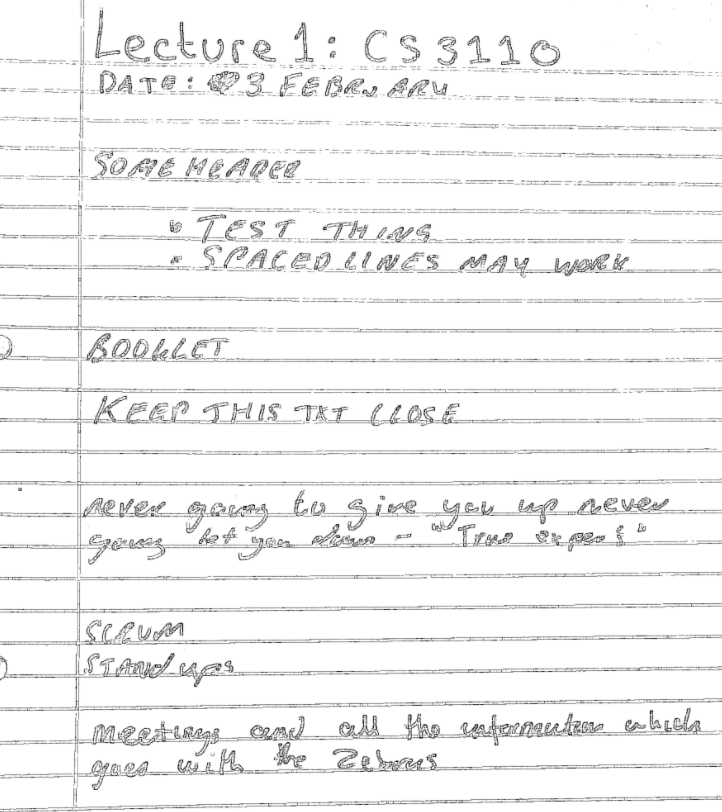
\includegraphics[scale=0.7]{images/pre-line-editing}
  \caption{The adaptive threshold on normal lined paper caused too much noise to be interfered with the Tesseract engine}
  \label{fig:pre-line-editing}
\end{figure}

\section{Filtering the blue lines}
\label{processing:filter_blue}
\begin{figure}[H]
  \centering
  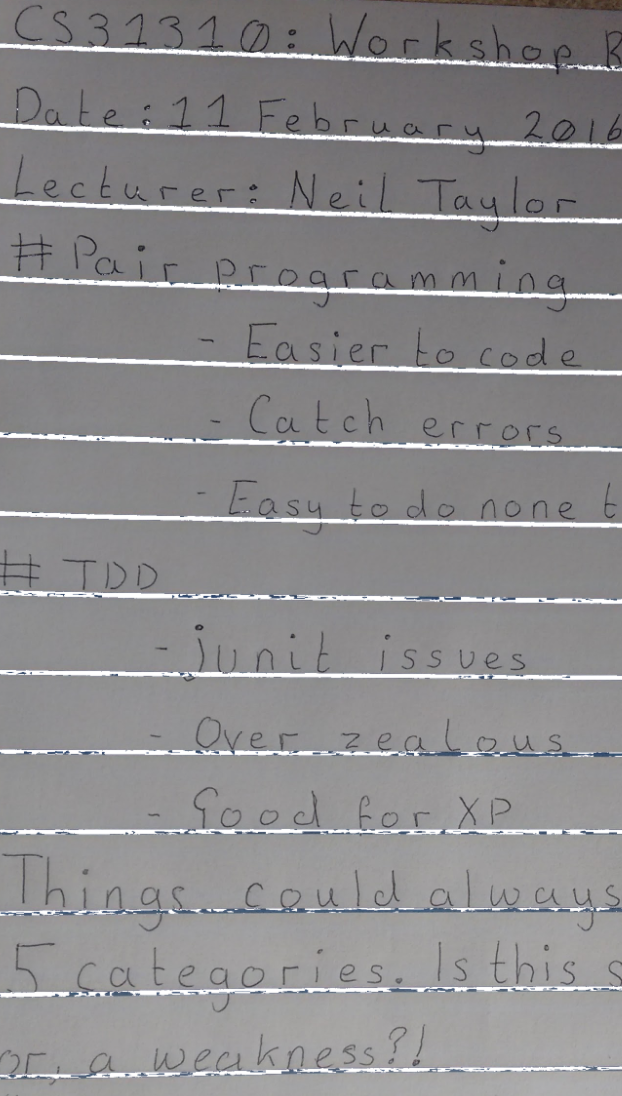
\includegraphics[scale=0.7]{images/blue_identified}
  \caption{Blue lines in the adaptive threshold have been identified and removed to be a white colour.}
  \label{fig:blue-identified}
\end{figure}
%TC:endignore
